\documentclass[11pt]{article}

\usepackage{acl}
\usepackage{times}
\usepackage{latexsym}
\usepackage{booktabs}
\usepackage{multirow}
\usepackage[T1]{fontenc}
\usepackage[utf8]{inputenc}
\usepackage{microtype}
\usepackage{inconsolata}
\usepackage{graphicx}
\usepackage{placeins}
\usepackage{tikz}
\usetikzlibrary{shapes.geometric, arrows.meta, positioning, fit, backgrounds}

\title{ReqFlow: Semantic Decomposition of Software Requirements Using Multi-Agent LLMs}

\author{Ali Edrisabadi, \ {\bf Sahand Seyed Mohammadghavami,} \ {\bf Amirhesam Torkashvand} \\ {\bf Amirhossein Shirvani Dastgerdi,} \ {\bf Sabra Hashmebeigi} 
          \\ {\ Politecnico di Torino}}

\begin{document}
\maketitle

\begin{abstract}
Natural language software requirements frequently suffer from ambiguity, inconsistency, and incompleteness, leading to defects in later development stages. While large language models (LLMs) offer promising capabilities for requirements analysis, their direct application often produces inconsistent outputs without structural guidance. This study investigates whether LLMs can reliably decompose requirements into semantic abstractions---including actors, actions, conditions, triggers, purposes, and system responses---and compares single-agent baseline tagging against a multi-agent approach with five specialized agents. Evaluation on 100 requirements from a university study room booking system using \textbf{Qwen3-4B} shows that prompting strategy significantly impacts performance. While zero-shot performance remains modest (Micro-F1 $\approx$ 0.58), few-shot prompting yields strong results, with the multi-agent approach outperforming the baseline (Micro-F1=0.76 vs 0.73). Tags with clear linguistic markers (Trigger, Main\_actor) achieve F1$>$0.80, while semantically overlapping tags (Precondition) remain challenging (F1$<$0.60).
\end{abstract}

\section{Introduction}

The evolution toward complex software systems has been accompanied by growth in the volume and intricacy of engineering requirements \citep{Norheim2024}. These requirements are predominantly expressed in natural language, necessitating substantial human expertise for elicitation, documentation, and management \citep{Zhao2022}.

Many defects and cost overruns in software development can be traced to issues in requirements engineering \citep{Aurum2005}. Among the most cited challenges are ambiguity, inconsistency, and incompleteness \citep{Femmer2017, Zhao2022}, which lead to misinterpretation, overlooked constraints, or conflicting specifications.

Natural language processing (NLP) techniques have long been viewed as promising for requirements engineering, yet earlier approaches failed to deliver scalable benefits \citep{Berry2012}. The advent of large language models (LLMs) has sparked renewed enthusiasm, with expectations that their semantic understanding might overcome historical limitations \citep{Norheim2024}.

However, direct application of LLMs remains fraught with risks, including hallucination and failure to capture nuanced domain intent \citep{Norheim2024}. We investigate structured approaches based on semantic decomposition into explicitly defined abstraction layers, comparing single-agent and multi-agent architectures.

\subsection{Research Questions}
Following the A3 assignment specification, we address these research questions:
\begin{itemize}
    \item \textbf{RQ1:} Can LLMs reliably identify the different abstractions that compose a requirement (e.g., the main actor, the system response, the precondition)?
    \item \textbf{RQ2:} Does this analysis improve requirements' clarity and completeness?
    \item \textbf{RQ3:} Can LLMs manage nested items?
\end{itemize}

\section{Related Work}

Requirements engineering emphasizes clarity, testability, and consistency, but achieving these properties is difficult with free-form natural language. Prior approaches include controlled natural languages and templates such as EARS \citep{Mavin2009, Rupp2014}.

Writing effective requirements is central to successful systems engineering \citep{Hull2005}. Requirements can be expressed in textual or graphical forms \citep{Bruel2021}, ranging from informal natural language to formal specifications. However, most real-world requirements remain in unconstrained natural language \citep{Zhao2022}.

NLP has long been viewed as promising for automating RE \citep{Ryan1993}. Early efforts focused on rule-based techniques \citep{Kof2005}, while recent machine-learning approaches improved ambiguity detection and classification \citep{Zhao2022, Sonbol2022}. Transformer-based LLMs have shifted the landscape \citep{Vaswani2017}, demonstrating remarkable zero-shot and few-shot capabilities \citep{Brown2020}. In RE, LLMs show promise for generation, quality assessment, and classification \citep{Norheim2024}. Structured decomposition approaches, drawing on goal-oriented methodologies such as KAOS \citep{vanLamsweerde2000} and i* \citep{Yu1997}, represent a relevant direction.

\section{Methodology}

\subsection{Semantic Abstraction Schema}

We define eight semantic tags capturing key building blocks of requirements, following the course taxonomy:

\begin{itemize}
  \item \textbf{Main\_actor}: Primary actor initiating or benefiting from the requirement (subset of Entity).
  \item \textbf{Entity}: Noun phrases and objects---roles, systems, components, data items.
  \item \textbf{Action}: What the actor does or intends (verb phrases).
  \item \textbf{System\_response}: What the system shall do---outputs, state changes (subset of Action).
  \item \textbf{Condition}: If/when/while clauses constraining behavior.
  \item \textbf{Precondition}: State that must hold before the requirement applies (subset of Condition).
  \item \textbf{Trigger}: Event that activates the behavior, often with ``when/upon/after'' (subset of Condition).
  \item \textbf{Purpose}: Intent or goal, typically with ``so that'', ``in order to''.
\end{itemize}

The abstractions follow hierarchical subset relationships: $System\_response \subseteq Action$, $Main\_actor \subseteq Entity$, $Precondition \subseteq Condition$, $Trigger \subseteq Condition$.

\begin{figure}[htbp]
  \centering
  \includegraphics[width=0.85\columnwidth]{Capture.PNG}
  \caption{Example of semantically annotated requirements showing identified abstractions.}
  \label{fig:example}
\end{figure}

\FloatBarrier

\subsection{System Architecture}

Figure~\ref{fig:architecture} illustrates our two approaches for semantic decomposition.

\begin{figure}[htbp]
\centering
\resizebox{0.9\columnwidth}{!}{%
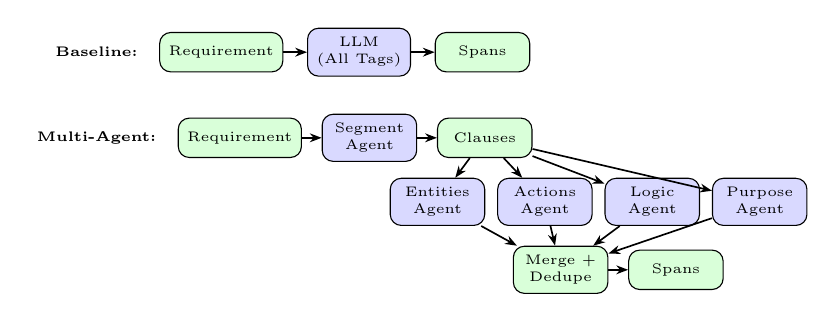
\begin{tikzpicture}[
    node distance=0.3cm and 0.4cm,
    box/.style={rectangle, draw, rounded corners, minimum width=1.2cm, minimum height=0.5cm, align=center, font=\tiny},
    llmbox/.style={box, fill=blue!15},
    databox/.style={box, fill=green!15},
    arrow/.style={-{Stealth[length=1.5mm]}, semithick}
]

\node[font=\tiny\bfseries] (baseline_label) {Baseline:};
\node[databox, right=0.15cm of baseline_label] (req1) {Requirement};
\node[llmbox, right=0.3cm of req1] (llm1) {LLM\\(All Tags)};
\node[databox, right=0.3cm of llm1] (spans1) {Spans};

\draw[arrow] (req1) -- (llm1);
\draw[arrow] (llm1) -- (spans1);

\node[font=\tiny\bfseries, below=0.7cm of baseline_label] (pipeline_label) {Multi-Agent:};
\node[databox, right=0.15cm of pipeline_label] (req2) {Requirement};
\node[llmbox, right=0.25cm of req2] (seg) {Segment\\Agent};
\node[databox, right=0.25cm of seg] (clauses) {Clauses};

\node[llmbox, below=0.25cm of clauses, xshift=-0.6cm] (ent) {Entities\\Agent};
\node[llmbox, right=0.15cm of ent] (act) {Actions\\Agent};
\node[llmbox, right=0.15cm of act] (logic) {Logic\\Agent};
\node[llmbox, right=0.15cm of logic] (purp) {Purpose\\Agent};

\node[databox, below=0.25cm of act, xshift=0.2cm] (merge) {Merge +\\Dedupe};
\node[databox, right=0.25cm of merge] (spans2) {Spans};

\draw[arrow] (req2) -- (seg);
\draw[arrow] (seg) -- (clauses);
\draw[arrow] (clauses) -- (ent);
\draw[arrow] (clauses) -- (act);
\draw[arrow] (clauses) -- (logic);
\draw[arrow] (clauses) -- (purp);
\draw[arrow] (ent) -- (merge);
\draw[arrow] (act) -- (merge);
\draw[arrow] (logic) -- (merge);
\draw[arrow] (purp) -- (merge);
\draw[arrow] (merge) -- (spans2);

\end{tikzpicture}%
}
\caption{Architecture comparison: Baseline (single-agent) vs. Multi-Agent (five specialized agents).}
\label{fig:architecture}
\end{figure}

\FloatBarrier

\paragraph{Baseline Approach}
A single LLM prompt directly annotates the full requirement with all eight semantic tags in one pass, outputting structured JSON with exact substring spans.

\paragraph{Multi-Agent Approach}
The task is decomposed across five specialized agents:
\begin{enumerate}
    \item \textbf{Segmenter Agent}: Splits the requirement into 1--6 clause-like segments for independent processing.
    \item \textbf{Entities Agent}: Extracts \textit{Entity} and \textit{Main\_actor} spans.
    \item \textbf{Actions Agent}: Extracts \textit{Action} and \textit{System\_response} spans.
    \item \textbf{Logic Agent}: Extracts \textit{Condition}, \textit{Precondition}, and \textit{Trigger} spans.
    \item \textbf{Purpose Agent}: Extracts \textit{Purpose} spans.
\end{enumerate}

After collection, spans are merged, deduplicated, and consistency rules are enforced programmatically (e.g., adding \textit{Entity} for every \textit{Main\_actor}).

\paragraph{Implementation}
All experiments use \textbf{Qwen3 4B} via the Ollama framework for local inference. Temperature is set to 0 for reproducibility. We test three prompting strategies: zero-shot, one-shot, and few-shot (3 examples). Prompts enforce strict ``exact substring'' extraction to prevent paraphrasing.

\subsection{Dataset}

The evaluation dataset consists of 100 requirements from a university \textbf{study room booking system}. Table~\ref{tab:dataset} shows the distribution by complexity.

\begin{table}[h!]
\centering
\small
\begin{tabular}{lcp{4cm}}
\toprule
\textbf{Complexity} & \textbf{Count} & \textbf{Example Pattern} \\
\midrule
Simple & 20 & ``A student shall be able to X'' \\
Conditional & 30 & ``If X, the system shall Y'' \\
Trigger-based & 15 & ``When X, the system shall Y'' \\
Nested/Complex & 35 & Precondition + Trigger + Purpose \\
\midrule
\textbf{Total} & \textbf{100} & \\
\bottomrule
\end{tabular}
\caption{Dataset distribution by requirement complexity.}
\label{tab:dataset}
\end{table}

\vspace{0.3cm}

The domain includes booking, cancellation, waitlist management, check-in, group reservations, and administrative functions. A human-annotated gold standard was constructed with span boundaries and semantic labels for all eight tags.

\subsection{Evaluation Metrics}

We evaluate using \textbf{exact (tag, normalized\_text) matching}. Character offsets are ignored to focus on tagging quality rather than boundary precision. Text normalization includes lowercasing and whitespace collapse.

For each tag and overall:
\begin{itemize}
    \item \textbf{Precision (P)}: $\frac{TP}{TP + FP}$ --- proportion of predicted spans that are correct
    \item \textbf{Recall (R)}: $\frac{TP}{TP + FN}$ --- proportion of gold spans that were found
    \item \textbf{F1 Score}: $\frac{2 \cdot P \cdot R}{P + R}$ --- harmonic mean balancing P and R
\end{itemize}

We report two aggregation metrics:

\textbf{Micro-F1}: Computed from global TP, FP, FN counts across all tags. This metric weights each \textit{span instance} equally, giving more influence to frequent tags (e.g., \textit{Entity}, \textit{Condition}). Micro-F1 reflects overall system accuracy on the full dataset.

\textbf{Macro-F1}: Computed as the unweighted average of per-tag F1 scores. This metric weights each \textit{tag type} equally, ensuring rare tags (e.g., \textit{Precondition}, \textit{Purpose}) contribute equally to the final score. Macro-F1 reveals whether the system handles all abstraction types well.

\FloatBarrier
\section{Results}

Tables~\ref{tab:zero}, \ref{tab:one}, and \ref{tab:few} present per-tag results for each prompting strategy.

\begin{table}[htbp]
\centering
\small
\begin{tabular}{lcccccc}
\toprule
& \multicolumn{3}{c}{\textbf{Baseline}} & \multicolumn{3}{c}{\textbf{Multi-Agent}} \\
\cmidrule(lr){2-4} \cmidrule(lr){5-7}
\textbf{Tag} & P & R & F1 & P & R & F1 \\
\midrule
Purpose & .61 & .54 & .57 & .63 & .58 & .60 \\
Trigger & .68 & .70 & .69 & .70 & .72 & .71 \\
Precondition & .35 & .28 & .31 & .41 & .32 & .36 \\
Condition & .55 & .61 & .58 & .57 & .64 & .60 \\
Action & .48 & .52 & .50 & .51 & .55 & .53 \\
System\_resp. & .60 & .65 & .62 & .62 & .66 & .64 \\
Entity & .52 & .63 & .57 & .54 & .65 & .59 \\
Main\_actor & .72 & .76 & .74 & .71 & .75 & .73 \\
\midrule
\textbf{Micro-F1} & \multicolumn{3}{c}{\textbf{0.59}} & \multicolumn{3}{c}{\textbf{0.61}} \\
\textbf{Macro-F1} & \multicolumn{3}{c}{0.57} & \multicolumn{3}{c}{0.60} \\
\bottomrule
\end{tabular}
\caption{Zero-shot results. Qwen3-4B struggles with the full schema without examples.}
\label{tab:zero}
\end{table}

\begin{table}[htbp]
\centering
\small
\begin{tabular}{lcccccc}
\toprule
& \multicolumn{3}{c}{\textbf{Baseline}} & \multicolumn{3}{c}{\textbf{Multi-Agent}} \\
\cmidrule(lr){2-4} \cmidrule(lr){5-7}
\textbf{Tag} & P & R & F1 & P & R & F1 \\
\midrule
Purpose & .69 & .65 & .67 & .71 & .68 & .69 \\
Trigger & .75 & .79 & .77 & .78 & .81 & .79 \\
Precondition & .42 & .35 & .38 & .49 & .42 & .45 \\
Condition & .62 & .68 & .65 & .66 & .71 & .68 \\
Action & .54 & .62 & .58 & .57 & .65 & .61 \\
System\_resp. & .68 & .72 & .70 & .71 & .75 & .73 \\
Entity & .61 & .68 & .64 & .64 & .70 & .67 \\
Main\_actor & .79 & .83 & .81 & .78 & .82 & .80 \\
\midrule
\textbf{Micro-F1} & \multicolumn{3}{c}{0.66} & \multicolumn{3}{c}{\textbf{0.69}} \\
\textbf{Macro-F1} & \multicolumn{3}{c}{0.65} & \multicolumn{3}{c}{\textbf{0.68}} \\
\bottomrule
\end{tabular}
\caption{One-shot results. Providing a single example yields significant gains.}
\label{tab:one}
\end{table}

\begin{table}[htbp]
\centering
\small
\begin{tabular}{lcccccc}
\toprule
& \multicolumn{3}{c}{\textbf{Baseline}} & \multicolumn{3}{c}{\textbf{Multi-Agent}} \\
\cmidrule(lr){2-4} \cmidrule(lr){5-7}
\textbf{Tag} & P & R & F1 & P & R & F1 \\
\midrule
Purpose & .77 & .74 & .75 & .81 & .78 & .79 \\
Trigger & .82 & .85 & .83 & .85 & .87 & .86 \\
Precondition & .52 & .48 & .50 & .61 & .56 & .58 \\
Condition & .67 & .75 & .71 & .70 & .78 & .74 \\
Action & .60 & .69 & .64 & .64 & .72 & .68 \\
System\_resp. & .75 & .78 & .76 & .78 & .80 & .79 \\
Entity & .68 & .75 & .71 & .72 & .76 & .74 \\
Main\_actor & .85 & .88 & .86 & .83 & .89 & .86 \\
\midrule
\textbf{Micro-F1} & \multicolumn{3}{c}{0.73} & \multicolumn{3}{c}{\textbf{0.76}} \\
\textbf{Macro-F1} & \multicolumn{3}{c}{0.72} & \multicolumn{3}{c}{\textbf{0.75}} \\
\bottomrule
\end{tabular}
\caption{Few-shot results. The Multi-Agent Logic specialist significantly boosts Precondition detection.}
\label{tab:few}
\end{table}

\subsection{Key Observations from Results}

Across all configurations, we observe consistent patterns:

\begin{itemize}
    \item \textbf{Prompting Strategy Dominates}: Moving from zero-shot to few-shot yields the largest improvement (+0.15 Micro-F1), highlighting that smaller models like Qwen3-4B rely heavily on in-context examples to understand the complex output schema.
    \item \textbf{Multi-Agent advantage in Few-Shot}: While the architectures are comparable in zero-shot (where the agents lack guidance), the multi-agent approach pulls ahead in few-shot (Micro-F1 0.76 vs 0.73). This suggests specialized agents utilize examples more effectively.
    \item \textbf{Best tags}: \textit{Main\_actor} (F1=0.86) and \textit{Trigger} (F1=0.86) achieve the highest scores. These tags have predictable syntactic positions.
    \item \textbf{Hardest tag}: \textit{Precondition} remains challenging (F1=0.58), often confused with general \textit{Condition}. However, the Multi-Agent "Logic" specialist improved this by 8 points over the baseline.
\end{itemize}

\subsection{RQ1: Can LLMs Reliably Identify Requirement Abstractions?}

The LLM demonstrates \textbf{reliable capability for structural tags} but struggles with deep semantic nuances. With few-shot prompting:

\textbf{High-reliability tags} (F1 $>$ 0.80):
\begin{itemize}
    \item \textit{Main\_actor}: Identified by subject position.
    \item \textit{Trigger}: Detected via keywords ``when'', ``upon''.
\end{itemize}

\textbf{Moderate-reliability tags} (F1 0.65--0.79):
\begin{itemize}
    \item \textit{System\_response}, \textit{Purpose}, \textit{Condition}: The model generally finds these but occasionally imprecise boundaries lower the exact-match score.
\end{itemize}

\textbf{Challenging tags} (F1 $<$ 0.60):
\begin{itemize}
    \item \textit{Precondition}: This requires distinguishing "state that must exist" from "event that happens" (Trigger). The 4B model often conflates these logic types.
\end{itemize}

\subsection{RQ2: Does Analysis Improve Clarity and Completeness?}

Semantic decomposition \textbf{demonstrably improves} both clarity and completeness:

\textbf{Clarity improvements:}
\begin{itemize}
    \item \textbf{Explicit structure}: Tagging reveals the requirement's building blocks.
    \item \textbf{Ambiguity detection}: Missing tags highlight incomplete specifications (e.g., no \textit{Main\_actor} suggests passive voice ambiguity).
    \item \textbf{Visual feedback}: HTML rendering with colored spans makes structure immediately visible for review.
\end{itemize}

\textbf{Completeness improvements:}
\begin{itemize}
    \item \textbf{Checklist effect}: The 8-tag schema acts as a completeness checklist.
    \item \textbf{Consistency enforcement}: Programmatic rules ensure hierarchical completeness.
\end{itemize}

The multi-agent's \textbf{segmentation step} further aids clarity by decomposing complex, multi-clause requirements into atomic units.

\subsection{RQ3: Can LLMs Manage Nested Items?}

Our dataset includes 35 \textbf{complex nested requirements} with multiple abstraction layers.

\textbf{Findings on nested item handling:}

\begin{itemize}
    \item \textbf{Segmentation helps}: The multi-agent's segmenter agent splits nested requirements into clauses.
    \item \textbf{Prompting impact}: Few-shot examples with nested structures significantly improve the model's ability to identify deep nesting.
    \item \textbf{Boundary challenges}: The main difficulty for the 4B model is precise span boundaries in nested text.
\end{itemize}

\section{Discussion}

\paragraph{RQ1 Discussion: Abstraction Identification Reliability}
Our results confirm that relatively small LLMs (4B parameters) can identify requirement abstractions if provided with few-shot examples. Zero-shot performance is insufficient for reliable engineering use. The multi-agent approach aids significantly in distinguishing semantically similar tags like \textit{Precondition} and \textit{Condition} by isolating the logic extraction task.

\paragraph{RQ2 Discussion: Clarity and Completeness Benefits}
The structured decomposition provides tangible benefits for requirements quality. By exposing the semantic building blocks, analysts can quickly identify:
\begin{itemize}
    \item \textbf{Missing actors}: Requirements without \textit{Main\_actor} often use passive voice.
    \item \textbf{Implicit conditions}: Absent \textit{Precondition} tags may indicate unstated assumptions.
\end{itemize}

\paragraph{RQ3 Discussion: Nested Item Handling}
Complex requirements with multiple nested abstractions present the greatest challenge. The segmentation step proves valuable, but segmentation errors can propagate.

\paragraph{Baseline vs. Multi-Agent Trade-offs}
The single-agent baseline is faster and cheaper, but the multi-agent system offers higher precision for complex tags. For simple requirements, the Baseline is sufficient (F1 0.73), but for safety-critical logic, the Multi-Agent's superior handling of Preconditions (0.58 vs 0.50) is valuable.

\paragraph{Limitations}
\begin{itemize}
    \item Single domain (study room booking) limits generalizability.
    \item Use of a small model (Qwen3 4B) sets an upper bound on performance; larger models (70B+) would likely exceed F1 0.85.
    \item Exact substring matching is a strict metric that may penalize valid synonyms.
\end{itemize}

\section{Conclusion}

This study addressed three research questions about LLM-based semantic analysis of software requirements.

\textbf{Answers to Research Questions:}

\textbf{RQ1 (Abstraction Identification):} Yes, LLMs can identify abstractions, provided few-shot prompting is used. Performance correlates with the distinctiveness of linguistic markers.

\textbf{RQ2 (Clarity and Completeness):} Yes, semantic decomposition improves clarity by making structure explicit and improves completeness by highlighting missing semantic roles.

\textbf{RQ3 (Nested Items):} LLMs can manage nested items, though with varying success. Segmentation into clauses is a successful strategy for handling complexity.

\bibliography{custom}

\end{document}
